\documentclass[conference]{IEEEtran}
\IEEEoverridecommandlockouts
\usepackage{fontspec}
\usepackage{xeCJK}
\setmainfont{Liberation Serif}
\setCJKmainfont[Scale=1.08]{Noto Serif CJK SC}
\setCJKsansfont{Noto Sans CJK SC}
\linespread{1.10}

\usepackage{amsmath,amssymb,amsfonts}
\usepackage{graphicx}
\usepackage{booktabs}
\usepackage{xcolor}
\usepackage{url}
\usepackage{microtype}

\graphicspath{{figures/}}

\renewcommand{\IEEEkeywordsname}{关键词}
\begin{document}

\title{LCP-Nav：面向跨域视觉导航的潜在后果预测}

\author{
\IEEEauthorblockN{
安中华\IEEEauthorrefmark{1}，
刘建翔\IEEEauthorrefmark{1}，
杨云钊\IEEEauthorrefmark{1}，
郭宁雁\IEEEauthorrefmark{1}\IEEEauthorrefmark{2}}
\IEEEauthorblockA{
\IEEEauthorrefmark{1}\textit{北京邮电大学}\\
中国北京\\
\url{2294822424@qq.com}；\url{liujianxiang@bupt.edu.cn}\\
\url{2025140284@bupt.cn}；\url{guoningyan@bupt.edu.cn}}
\IEEEauthorblockA{\IEEEauthorrefmark{2}通讯作者：郭宁雁}
}

\maketitle

\begin{abstract}
视觉导航策略可以持续取得路线进度，却可能因局部误差不断累积而错过图像指定的目的地。直接回归单条局部轨迹的策略没有显式比较不同动作可能到达的终点。本文提出视觉导航潜在后果预测方法（Latent Consequence Prediction for Navigation，LCP-Nav）：生成有限条候选轨迹，利用共享的动作条件潜变量动力学递推每条候选轨迹，并选择预测终点与目标最一致的候选。跨域测试表明，LCP-Nav 在 ReCon 和 SCAND 上的动作损失低于 ViNT；重复 Gazebo 实验表明，在三条路线上的终点误差更低、经验证到达次数更多。LCP-Nav 包含 $26.77$~M 个参数，在 RTX~4090 上的 p95 延迟为 $24.8$~ms，推理速度保持在 $40$~Hz 以上。实验结果表明，潜变量终点比较可以作为视觉导航中有效且高效的决策层。
\end{abstract}

\begin{IEEEkeywords}
视觉导航，世界模型，潜变量动力学，移动机器人
\end{IEEEkeywords}

\section{引言}

视觉导航使移动机器人能够依据近期 RGB 观测和目标图像到达图像指定的目的地。现代策略从异构机器人轨迹中学习这一映射，并将其迁移到不同平台和环境~\cite{gnm,vint}。这类方法的性能通常通过路线进度或局部动作误差概括。然而，这两个量都不能直接描述机器人最终停在哪里。单个预测时域内看似很小的偏差可能逐渐累积，使机器人在走过大部分路线后仍远离目的地。

对于直接回归单条局部轨迹的策略，这一不匹配尤其明显。这类策略可以学习到较强的平均动作，但其输出不会显式呈现可选运动，也无法根据候选动作预测的终点状态进行区分。我们的闭环审计揭示了其实际后果：较高的拓扑进度可能与较大的终点误差同时出现。因此，提高到达可靠性需要一个与动作序列后果相关的决策变量，而不是对局部进度进行另一种估计。

两条局部轨迹在模仿损失下可能同样合理，却可能将机器人带到与目标关系不同的状态。一旦其中一条轨迹被执行，其位移和航向误差就会进入下一轮规划。保留多条可行动作并在执行前比较其可能到达的终点，为策略在误差发生之前规避误差提供了机会。

世界模型为后果感知决策提供了自然路径，但当决策只需要比较局部动作时，没有必要生成完整的未来 RGB 观测~\cite{nwm,uniwm}。紧凑的潜变量转移可以直接预测动作序列如何改变与任务相关的视觉状态。要让这一预测用于动作选择，需要满足两个条件：不同动作应产生可区分的潜变量终点，选择器应结合这些终点与目标之间的关系进行决策。

LCP-Nav 围绕这两个条件进行设计。确定性候选头提出 $K$ 条可行局部轨迹；共享的动作条件动力学将每条候选轨迹映射为想象终点；目标感知评分器从这些预测后果中进行选择。软候选监督使候选生成目标与排序目标保持一致，而 SIGReg 保持潜变量状态的变化，使终点比较具有信息量。未来观测只在训练阶段监督动力学；推理时仍使用与标准视觉策略相同的观测历史和目标图像。

候选头无需迭代采样即可产生多种动作，共享转移模型则在同一表示空间中评估这些动作。目标与终点之间的差异直接表示终点兼容性；非坍塌正则化则保持视觉上不同的状态彼此可区分。因此，LCP-Nav 改变了局部动作的选择方式，同时保留原有视觉输入和拓扑导航接口。

我们分别检验该设计中的各个环节。匹配的离线实验测量域内和跨域动作预测；递归 rollout 与终点置换测试判断学习到的动力学是否保持预测能力并影响选择；重复 Gazebo 运行测量终点误差和经验证到达；性能分析量化有限潜变量 rollout 的计算代价。这些证据将所提出的决策机制与跨域迁移和闭环行为联系起来。

\section{相关工作}

\textbf{通用视觉导航策略。} ViNG 将拓扑记忆引入视觉导航~\cite{ving}；GNM 统一了异构机器人数据~\cite{gnm}；ViNT 则将 Transformer 策略扩展到不同机器人平台~\cite{vint}。NoMaD 通过扩散模型和目标屏蔽建模多模态动作~\cite{nomad}，LiMo 则利用规划器生成的监督信号扩充有限示范数据~\cite{limo}。这些方法改善了迁移能力、数据效率或动作多样性，但其动作输出并未通过显式预测每个候选动作终点的方式进行选择。关于零样本导航和碰撞避免的评估也进一步说明，在视觉和几何条件发生变化时，需要保持决策可靠性~\cite{vfm-eval,care}。

\textbf{世界模型与潜变量预测。} Navigation World Models 生成动作条件的未来视图以支持规划~\cite{nwm}，UniWM 将视觉预见与自回归动作生成结合起来~\cite{uniwm}。ExploreVLA 使用未来 RGB 和深度作为自动驾驶的密集监督~\cite{explorevla}。LCP-Nav 只预测用于排序小规模确定性候选集所需的潜变量终点，从而不需要像素重建和迭代式动作采样。相关的联合嵌入模型在表示空间中稳定预测~\cite{lewm}；本文则将潜变量动力学与距离估计、轨迹生成和基于终点的选择联合训练。

\begin{figure*}[t]
\centering

\includegraphics[width=0.99\textwidth]{fig1_lcp_architecture_editable.png}
\caption{LCP-Nav 架构。六个观测 token 和一个当前图像--目标图像融合 token 输入四层 Transformer。共享表示分别输入 ViNT 风格的时间距离头和动作头，后者生成三条候选轨迹。潜变量动力学预测每条候选轨迹的后果，目标条件评分器选择实际执行的动作。训练期间，未来 RGB 帧通过同一个观测编码器；动力学损失训练共享潜变量 rollout，SIGReg 则对观测和未来嵌入进行正则化。实线箭头表示在线推理，琥珀色虚线箭头表示仅训练阶段使用的监督。}
\label{fig:architecture}
\end{figure*}

\section{方法}

\subsection{问题与架构}

我们将局部规划表述为在预测后果之间进行选择。在时刻 $t$，策略接收 $O_t=\{o_{t-P},\ldots,o_t\}$ 和目标图像 $o_g$。观测编码器和目标编码器形成 token，Transformer 将其融合为 $h_t$。候选头预测
\begin{equation}
\{\hat A_t^1,\ldots,\hat A_t^K\}=f_{\mathrm{cand}}(h_t),
\end{equation}
其中每条候选轨迹包含 $H$ 个航点。每个航点表示为 $a_i=(\Delta x_i,\Delta y_i,\cos\theta_i,\sin\theta_i)$。EfficientNet-B0 对六张观测图像以及当前图像--目标图像对进行编码。类型嵌入区分历史观测、当前观测和目标 token；正弦位置编码在四层 Transformer 编码器处理前保留其顺序。最终的观测 token 和目标 token 分别定义 $z_t$ 与 $z_g$，均值 token $h_t$ 则驱动候选头和时间距离头。候选头结合 $h_t$ 与可学习的候选身份，预测有界位置增量和归一化航向，并将这些增量累积为局部坐标系中的航点。图~\ref{fig:architecture} 区分了部署路径和仅训练阶段使用的监督。

\subsection{生成、想象与选择}

对于候选 $k$，轨迹误差由 Smooth-L1 位置误差和航向余弦距离组成，即 $e_k=e_k^{\mathrm{pos}}+\lambda_\theta e_k^\theta$。候选回归和排序使用软目标
\begin{equation}
w_k=\frac{e^{-e_k/\tau_a}}{\sum_j e^{-e_j/\tau_a}},\qquad
q_k=\frac{e^{-e_k/\tau_s}}{\sum_j e^{-e_j/\tau_s}},
\end{equation}
并令 $L_{\mathrm{reg}}=\sum_k w_ke_k$、$L_{\mathrm{score}}=-\sum_kq_k\log\operatorname{softmax}(s)_k$。完整的候选目标为
\begin{equation}
L_{\mathrm{cand}}=L_{\mathrm{reg}}+L_{\mathrm{score}}+0.1L_{\mathrm{smooth}}+0.05L_{\mathrm{step}}+0.02L_{\mathrm{div}}.
\end{equation}
平滑项和步长项抑制不稳定运动，$L_{\mathrm{div}}$ 则分离候选终点。软分配避免获胜候选发生突变，并为评分器提供与轨迹质量一致的排序目标。

回归损失按照候选质量分配监督，而不是只更新一个硬获胜候选；评分损失学习相同的排序关系。多样性间隔作用于最终位置，在不强制每个中间航点都不同的情况下保留不同候选终点。所有候选轨迹均在一次前向传播中生成。

\subsection{预测性训练与非坍塌正则化}

训练期间，专家动作驱动三步 teacher-forced rollout，真实未来帧提供停止梯度的目标。给定有效性掩码 $m_{b,h}$，动力学损失为
\begin{equation}
L_{\mathrm{dyn}}=\frac{\sum_{b,h}m_{b,h}[1-\cos(\hat z_{b,t+h},\operatorname{sg}(z_{b,t+h}))]}{\sum_{b,h}m_{b,h}}.
\end{equation}
单独的预测训练可能导致不同状态发生坍塌。为此，SIGReg 将观测 token 和未来 token 的一维随机投影与标准高斯分布进行匹配。对于 $Z\in\mathbb{R}^{B\times T\times D}$ 中的嵌入、单位投影 $r_m$、节点 $u_l$ 和 $W=\sum_l\omega_l$，计算
\begin{equation}
\begin{aligned}
L_{\mathrm{sig}}=\frac{1}{MW}\sum_{m,l}\omega_l\big[&\big(\mathbb{E}\cos(u_l Z^\top r_m)-e^{-u_l^2/2}\big)^2\\
&+\big(\mathbb{E}\sin(u_l Z^\top r_m)\big)^2\big].
\end{aligned}
\end{equation}
期望在 batch 和时间 token 上取平均。匹配投影后的特征函数，可以避免模型通过近似恒定的表示取得较低预测损失。完整训练目标为
\begin{equation}
L=\bar L_{\mathrm{dist}}+\bar L_{\mathrm{cand}}+\gamma(e)\bar L_{\mathrm{dyn}}+\lambda_{\mathrm{sig}}L_{\mathrm{sig}},
\end{equation}
其中上划线表示除以对应损失幅值的指数移动平均，$\gamma(e)$ 按 epoch 逐步增加动力学项的权重。$L_{\mathrm{dist}}$ 是目标时间距离的 Smooth-L1 误差。训练时，未来观测只作为潜变量目标；部署时只需要观测历史、目标图像和候选动作。

\begin{figure*}[t]
\centering
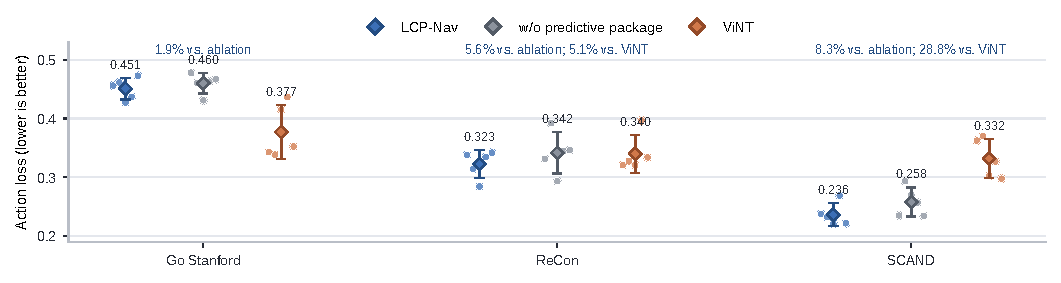
\includegraphics[width=0.98\textwidth]{fig2_offline_multiseed.pdf}
\caption{五个随机种子的离线动作损失（点），以及均值 $\pm$ 样本标准差（菱形和误差条）。所有检查点均依据 Go Stanford 验证数据选择；ReCon 和 SCAND 是只使用检查点的零样本测试。预测路径消融在其他训练设置匹配的情况下移除想象终点、潜变量 rollout 和动力学监督。}
\label{fig:offline}
\end{figure*}

\section{实验}

\subsection{实验设置}

\textbf{离线评估。} LCP-Nav、匹配的预测路径消融模型和 ViNT 在 Go Stanford 上分别使用五个随机种子独立训练。消融模型保留输入、骨干网络、动作接口、数据和优化预算，但移除想象终点、动作条件 rollout 和动力学监督。依据验证集选择的检查点在固定的 Go Stanford、ReCon 和 SCAND 样本上进行评估；ReCon 和 SCAND 不进行微调，也不重新选择目标域数据。每次完整训练运行作为一次重复实验（$n=5$），各随机种子的结果给出图~\ref{fig:offline} 中的不确定性。

所有模型使用 $96\times96$ RGB 输入、六张观测图像、五个预测航点、512 维视觉特征和四层 Transformer 编码器。LCP-Nav 使用 $K=3$、$\lambda_\theta=1$、$\tau_a=\tau_s=1$、$\lambda_{\mathrm{sig}}=0.12$、三步监督动力学时域、1024 个 SIGReg 投影和 17 个特征函数节点。动力学权重在前五个 epoch 中为零，在 epoch 5--10 之间线性增加到一，此后保持为一。AdamW 训练 15 个 epoch，batch size 为 128，初始学习率为 $8\times10^{-4}$，采用余弦调度。数据、测试样本和优化预算均保持匹配。离线动作损失取航点 Smooth-L1 损失和航向余弦损失的平均值。

验证集动作损失用于选择 LCP-Nav-action 和 ViNT，以进行动作比较。验证集潜变量预测损失用于选择 LCP-Nav-LFP，以进行 rollout 分析和 Gazebo 部署。测试集和 Gazebo 结果不参与检查点选择。

\textbf{闭环评估。} Gazebo 实验使用固定的室内障碍、林间道路和校园道路路线，分别测试受限通道、外观变化和长时域漂移。每种方法在每条路线运行五次。相机、底盘、控制器、拓扑图、起始位姿和到达检测器均保持不变。经验证到达需要同时满足软件报告到达、终点误差不超过 5~m、无碰撞且未超时。终点误差是机器人与示范终点之间的欧氏距离；拓扑进度是到达的最大节点索引除以目标节点索引。每次重复实验都是一次完整运行，其中包括碰撞和超时。

\begin{figure*}[t]
\centering
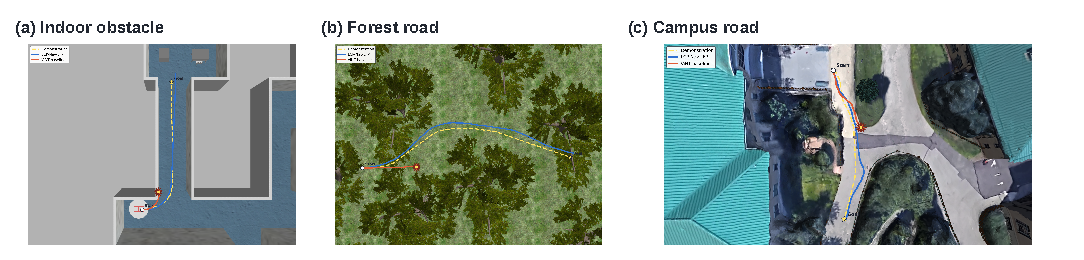
\includegraphics[width=0.96\textwidth]{fig3_overhead_scene_context.pdf}
\vspace{0.35em}
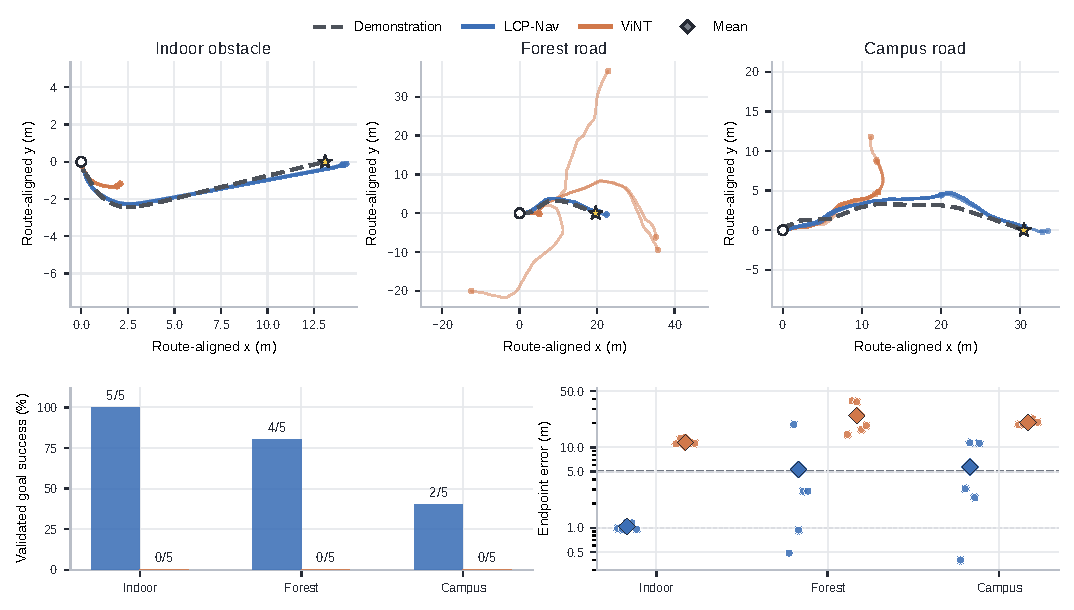
\includegraphics[width=0.96\textwidth,trim=0 0 0 175bp,clip]{fig3_closed_loop_simulation.pdf}
\caption{场景驱动的闭环 Gazebo 评估。路线分别考察受限通道、外观变化和终点漂移。上图：(a) 室内障碍路线，(b) 林间道路路线，(c) 校园道路路线的俯视图；黄色虚线为示范路线，蓝色和橙色分别为保留的 LCP-Nav 与 ViNT 轨迹，圆圈表示起点，星号表示示范终点，爆裂符号表示失败停止位置。下图：每种方法和场景下五次运行的经验证到达和终点误差（菱形表示均值；终点误差使用对数坐标；虚线标记 1~m 和 5~m）。}
\label{fig:simulation}
\end{figure*}

\subsection{跨域迁移与机制分析}

预测路径在发生域偏移后带来的收益最为明显。相对于匹配的消融模型，LCP-Nav 在 Go Stanford、ReCon 和 SCAND 上分别将平均动作损失降低 1.9\%、5.6\% 和 8.3\%（图~\ref{fig:offline}）。在 Go Stanford 测试集上，ViNT 仍然更优（0.3771 对比 0.4510）；而在 ReCon（0.3226 对比 0.3399）和 SCAND（0.2363 对比 0.3319）上，LCP-Nav 的损失更低。SCAND 的每个随机种子均优于 ViNT；配对均值差为 $-0.0955$，95\% 穷举 bootstrap 区间为 $[-0.1228,-0.0698]$。完整模型相对于匹配消融模型的增益逐渐扩大，说明当外观和运动统计偏离训练域时，潜在后果预测的作用更加明显。

Go Stanford、ReCon 和 SCAND 的航点间距分别为 0.12、0.25 和 0.38~m。以物理单位表示的组成指标揭示了总体收益如何随域变化。在 ReCon 上，LCP-Nav 将平移 RMSE 从 0.333~m 降至 0.325~m，而 ViNT 的角度误差更低（0.264 对比 0.290~rad）。在 SCAND 上，LCP-Nav 的平移 RMSE 略高（0.555 对比 0.546~m），但将角度误差从 0.162 降至 0.122~rad。因此，动作损失的改善并不是每个组成项都统一下降，而是反映了域偏移下平移和航向之间不同的平衡。数据划分审计未发现训练集与测试集之间存在轨迹交集，也未发现 Go Stanford 验证轨迹与测试轨迹之间存在重叠。

机制测试解释了这一现象。在 $\lambda_{\mathrm{sig}}=0.12$ 时，三条候选轨迹的动作损失为 0.3919，低于一条候选轨迹的 0.4318 和五条候选轨迹的 0.4685。移除 SIGReg 后，潜变量预测损失降至 0.0023，但有效秩坍塌至 1.02，且第一特征值解释了 99.7\% 的方差。因此，当不同观测几乎映射到同一个潜变量状态时，较低的预测误差并不能提供有效信息。相反，仅对想象终点进行循环置换，会改变三个数据集上约 43\% 的候选选择，说明评分器确实利用了终点表示。

递归 rollout 下，转移模型仍然保留了有用结构。一、二、三步潜变量 MSE 分别为 1.653、2.318 和 2.732，而匹配消融模型分别为 3.743、4.195 和 4.604。在第三步，预测性检查点的余弦一致性仍为 $0.9024\pm0.0387$，而消融模型降至 $0.5098\pm0.0529$。秩、rollout 和终点干预的联合证据确定了一条功能链：SIGReg 保持状态差异，动力学在候选动作下传播这些差异，评分器再利用生成的终点进行选择。

候选数量扫描明确了 $K$ 的选择。一条候选轨迹不给终点评分器留下选择空间，而五条候选轨迹会将监督分散到更多假设上，并提高动作损失。三条候选轨迹能够提供终点变化，同时保持每个候选得到充分监督。

\subsection{闭环到达与效率}

LCP-Nav 将迁移收益转化为更可靠的闭环终止。在室内、林间和校园路线中，LCP-Nav 分别取得 5/5、4/5 和 2/5 次经验证到达，而 ViNT 在每个场景中均为 0/5（图~\ref{fig:simulation} 和表~\ref{tab:closedloop}）。LCP-Nav 的平均终点误差分别为 1.04、5.30 和 5.70~m，ViNT 则为 11.56、24.91 和 20.40~m。俯视图定位了相应的失败位置：ViNT 在受限的室内通道附近停止，在林间路线更早偏离，并在校园路线到达最终节点后仍未在终点附近终止。

\begin{table}[t]
\centering
\caption{重复闭环仿真（均值 $\pm$ 样本标准差；每种方法和场景 $n=5$ 次运行）。}
\label{tab:closedloop}
\setlength{\tabcolsep}{3.2pt}
\footnotesize
\begin{tabular}{@{}llccc@{}}
\toprule
场景 & 方法 & 到达 & 误差（m） & 进度（\%） \\
\midrule
室内 & LCP-Nav & 5/5 & $1.04\pm0.10$ & $100.0\pm0.0$ \\
     & ViNT    & 0/5 & $11.56\pm0.83$ & $48.2\pm27.3$ \\
林间 & LCP-Nav & 4/5 & $5.30\pm7.93$ & $79.2\pm42.1$ \\
     & ViNT    & 0/5 & $24.91\pm11.43$ & $44.8\pm11.4$ \\
校园 & LCP-Nav & 2/5 & $5.70\pm5.24$ & $83.8\pm17.5$ \\
     & ViNT    & 0/5 & $20.40\pm1.42$ & $100.0\pm0.0$ \\
\bottomrule
\end{tabular}
\end{table}

按场景划分的结果将路线遍历与终点准确性区分开来。在室内场景中，LCP-Nav 在受限通道中稳定成功。外观变化导致林间路线出现一次大误差运行，而更长的校园路线仍有两次不准确终止。ViNT 在校园场景中最清楚地体现了指标不匹配：它达到 100\% 的平均拓扑进度，却距离终点 $20.40\pm1.42$~m。采用更严格的 1-m 阈值时，LCP-Nav 有 6/15 次运行、ViNT 有 0/15 次运行仍属于有效到达，方法排序保持不变。

俯视轨迹区分了两类失败模式。室内和林间的 ViNT 运行会偏离或提前停止，而校园基线虽然沿着节点序列前进，却逐渐积累了相对于终点的物理位移。LCP-Nav 在每次室内运行中都通过了瓶颈，并在大多数林间和校园运行中将终止位置控制在 5-m 标准以内；其剩余的大误差运行出现在两条较长路线中。

策略级性能分析使用 100 次预热迭代，随后进行 500 次计时重复。LCP-Nav 包含 $26.77$~M 个参数，比 ViNT 少 9.8\%，约需要 $1.164$~GFLOPs。在 RTX~4090、float32 输入下，其 p95 延迟为 24.3--24.8~ms，而 ViNT 为 22.6~ms；峰值分配内存为 129.6--131.3~MiB，而 ViNT 为 142.7~MiB。因此，三次潜变量 rollout 仅增加 1.7--2.2~ms，同时保持 $40$~Hz 以上的推理速度。

\enlargethispage{-1.25in}
\section{讨论}

实验表明，轨迹生成和轨迹选择解决的是视觉导航中的两个不同问题。直接回归可以产生局部上合理的动作，却没有依据在会到达不同终点状态的动作之间进行选择。LCP-Nav 将这一选择显式化。匹配消融实验表明，跨域收益的增加来自预测路径；终点干预则确认，当想象后果发生变化时，评分器会改变其决策。候选多样性本身并不足够：如果潜变量状态发生坍塌，较低的预测误差就无法为排序提供有效信息。

ViNT 在 Go Stanford 上更准确地拟合动作，而 LCP-Nav 使用相同源数据，却在 ReCon 和 SCAND 上反转了这一排序。结合匹配消融结果，这一模式表明，预测路径带来的贡献并非仅来自模型容量。组成指标显示的是具有域特异性的权衡，而不是统一的平滑效果：在两个目标域中，平移和航向误差的变化并不相同。

闭环行为使这一差异更加直观。室内结果表明，终点评分可以选择穿过受限通道的稳定运动；林间结果表明，该优势在外观变化下仍然存在。校园路线更加困难：LCP-Nav 显著降低了终点误差，但随着更长路线上的误差累积，仍有若干次终止不够准确。ViNT 到达了每个校园节点，却停在远离目的地的位置，说明拓扑进度必须与终点误差和经验证到达结合使用。LCP-Nav 只增加了少量延迟，因此基于后果的动作选择仍然适用于实时控制。

\section{结论}

LCP-Nav 在动作执行前比较有限条局部轨迹的预测潜变量后果，以缓解视觉导航中的终点漂移。在 ReCon 和 SCAND 上，其动作损失低于 ViNT；在三条闭环 Gazebo 路线中，其终点误差更低、经验证到达次数更多，同时保持 $40$~Hz 以上的推理速度。这些结果表明，基于终点的后果比较能够在不牺牲实时控制能力的情况下改善动作选择。

\begin{thebibliography}{00}
\bibitem{ving} D. Shah, B. Eysenbach, G. Kahn, N. Rhinehart, and S. Levine, \textquotedblleft ViNG: Learning open-world navigation with visual goals,\textquotedblright{} in \emph{Proc. IEEE Int. Conf. Robot. Autom.}, 2021.
\bibitem{gnm} D. Shah, A. Sridhar, A. Bhorkar, N. Hirose, and S. Levine, \textquotedblleft GNM: A general navigation model to drive any robot,\textquotedblright{} in \emph{Proc. IEEE Int. Conf. Robot. Autom.}, 2023.
\bibitem{vint} D. Shah \emph{et al.}, \textquotedblleft ViNT: A foundation model for visual navigation,\textquotedblright{} in \emph{Proc. Conf. Robot Learn.}, vol. 229, pp. 711--733, 2023.
\bibitem{nomad} A. Sridhar, D. Shah, C. Glossop, and S. Levine, \textquotedblleft NoMaD: Goal masked diffusion policies for navigation and exploration,\textquotedblright{} arXiv:2310.07896, 2023.
\bibitem{vfm-eval} M. Guerrier, K. Soma, J. Pavlasek, and G. Beltrame, \textquotedblleft Can vision foundation models navigate? Zero-shot real-world evaluation and lessons learned,\textquotedblright{} arXiv:2603.25937, 2026.
\bibitem{care} J. Kim, J. Sim, W. Kim, K. Sycara, and C. Nam, \textquotedblleft CARE: Enhancing safety of visual navigation through collision avoidance via repulsive estimation,\textquotedblright{} in \emph{Proc. 9th Conf. Robot Learn.}, 2025.
\bibitem{limo} Y. Inglin, J. Frey, C. Chen, and M. Hutter, \textquotedblleft Less is more: Scalable visual navigation from limited data,\textquotedblright{} arXiv:2601.17815, 2026.

\bibitem{nwm} A. Bar, G. Zhou, D. Tran, T. Darrell, and Y. LeCun, \textquotedblleft Navigation world models,\textquotedblright{} arXiv:2412.03572, 2024.
\bibitem{uniwm} Y. Dong \emph{et al.}, \textquotedblleft Unified world models: Memory-augmented planning and foresight for visual navigation,\textquotedblright{} arXiv:2510.08713, 2025.
\bibitem{explorevla} Z. Sheng, X. Ye, J. Luo, S. Chen, and L. Ren, \textquotedblleft ExploreVLA: Dense world modeling and exploration for end-to-end autonomous driving,\textquotedblright{} arXiv:2604.02714, 2026.
\bibitem{lewm} L. Maes, Q. Le Lidec, D. Scieur, Y. LeCun, and R. Balestriero, \textquotedblleft LeWorldModel: Stable end-to-end joint-embedding predictive architecture from pixels,\textquotedblright{} arXiv:2603.19312, 2026.
\end{thebibliography}

\end{document}
